\documentclass[10pt,conference]{IEEEtran}

\usepackage[utf8]{inputenc}
\usepackage{amsmath,amsfonts,amssymb}
\usepackage{booktabs}
\usepackage{graphicx}
\usepackage{hyperref}
\usepackage{algorithm}
\usepackage{algpseudocode}
\usepackage{cite}
\usepackage{xcolor}
\usepackage{array}
\usepackage{subfig}
\usepackage{placeins}
\graphicspath{{images/}}

\hypersetup{colorlinks=true, linkcolor=blue, citecolor=blue, urlcolor=blue}

\title{%
  Enhancing Heuristic and Metaheuristic Solutions for \\ 
  the Weapon-Target Assignment Problem via \\
  Iterative Refinement and Hybrid Genetic Algorithms
}

\author{%
  \IEEEauthorblockN{%
    Most.\ Sonia Khatun,\;
    Ahmmad Nur Swapnil,\;
    Sadia Tabassum,\;
    Hozifa Rahman Hamim,\;
    Md.\ Azizul Haque Nadim
  }
  \IEEEauthorblockA{%
    Department of Computer Science and Engineering\\
    Bangladesh University of Engineering and Technology (BUET)\\
    Dhaka, Bangladesh\\
    \\
    Course Supervisors: Nafis Tahmid and Mohammad Sadat Hossain\\
    Lecturers, Department of CSE, BUET
  }
}

\begin{document}

\maketitle

% ─────────────────────────────────────────────────────────────────────────────
\begin{abstract}
The Weapon-Target Assignment (WTA) problem asks how to allocate a finite set of
weapons to a set of targets so as to minimise the expected total survival value
of those targets.  It is NP-complete, and recent exact methods have improved
scalability for centralized static instances \cite{bertsimas2025}.  In
practice, however, many deployments still require lightweight methods with
predictable runtime under strict decision windows and constrained compute.
This paper presents two algorithm engineering contributions.  First, we augment the
classic Maximum Marginal Return (MMR) greedy heuristic with (i) tie-breaking
by current target value, (ii) a 1-opt iterative local-search pass, and
(iii) a 2-opt swap-search pass, yielding the MMR-IR algorithm.  Second, we redesign the
standard Genetic Algorithm (GA) with (i) MMR-seeded initialisation,
(ii) elitism with stagnation-triggered re-diversification, and
(iii) threat-proportional mutation, yielding the Hybrid GA.
Both modifications are evaluated on a structured synthetic benchmark of
180 instances spanning nine categories (three size tiers $\times$ three
weapon-availability scenarios).
MMR-IR improves MMR in all nine categories, with per-category gains ranging
from $0.11\%$ to $3.15\%$.
On balanced instances, MMR-IR improves MMR by $2.44\%$, $0.46\%$, and
$0.13\%$ in small, medium, and large tiers, respectively.
Hybrid GA changes GA performance by $-2.95\%$, $28.73\%$, and $37.42\%$ in the
same tiers, showing strong gains at medium/large scale but mixed small-tier
behaviour.
Using Wilcoxon signed-rank tests ($\alpha = 0.05$, alternative = greater),
MMR-IR is significant in $9/9$ categories and Hybrid GA in $6/9$ categories
(all three small-tier categories are non-significant for Hybrid GA).
\end{abstract}

\begin{IEEEkeywords}
Weapon-Target Assignment, greedy heuristic, genetic algorithm, iterative refinement, local search, combinatorial optimisation
\end{IEEEkeywords}

% ─────────────────────────────────────────────────────────────────────────────
\section{Introduction}

The Weapon-Target Assignment (WTA) problem is a central combinatorial
optimisation problem in military operations research.  Given a set of weapons
and a set of incoming targets, each weapon-target pair is characterised by a
kill probability $p_{ij}$, and each target carries a strategic value $V_j$.
The objective is to find an integer allocation $x_{ij}$ (number of weapons of
type $i$ assigned to target $j$) that minimises the expected residual threat
$\sum_j V_j \prod_i (1-p_{ij})^{x_{ij}}$, subject to weapons not exceeding their
available stock.

Operational WTA settings often require high-quality assignments within tight
decision windows, so the trade-off between solution quality and runtime remains
central in practice \cite{kline2020}.

Recent branch-price-and-cut methods show that centralized exact optimization can
scale to very large static WTA instances \cite{bertsimas2025}.  Our focus is
therefore complementary: we target settings where lightweight implementations,
low overhead, and bounded runtime are preferred, such as compute-constrained or
time-critical deployments.

WTA belongs to the class of NP-complete problems \cite{ahuja2007,lloyd1986},
so practical systems often combine exact methods (when centralized resources
permit) with heuristics and metaheuristics for fast decision-making.
Two widely studied baseline heuristic/metaheuristic approaches are the
Maximum Marginal Return (MMR) greedy heuristic and a Genetic Algorithm (GA)
\cite{ahuja2007,kline2020}.  MMR is extremely fast but commits irrevocably to
early greedy choices.  Standard GA explores the solution space more broadly
but suffers from slow convergence, solution loss between generations, and
uninformed mutation in large-dimensional instances.

This paper makes the following contributions:

\begin{itemize}
  \item We propose \textbf{MMR-IR}, an extension of MMR that adds tie-aware
        greedy allocation followed by 1-opt and 2-opt local search, with
        $O(1)$ incremental objective evaluation per trial.
  \item We propose \textbf{Hybrid GA}, which addresses three identified
        weaknesses of standard GA through MMR-seeded initialisation, elitism
      with stagnation-triggered re-diversification, and a
        threat-proportional mutation operator.
  \item We design and open-source a structured 180-instance synthetic
        benchmark covering small, medium, and large problem sizes under
        balanced, scarce, and weapon-rich resource scenarios.
  \item We provide a comprehensive experimental evaluation including
        one-sided Wilcoxon signed-rank testing; MMR-IR is significant in
        $9/9$ categories, while Hybrid GA is significant in $6/9$ and shows
        its strongest gains on medium and large tiers.
\end{itemize}

The remainder of the paper is organised as follows.
Section~\ref{sec:problem} formalises the WTA problem and summarises its
complexity status.
Section~\ref{sec:survey} surveys existing solution approaches.
Sections~\ref{sec:mmr} and~\ref{sec:ga} describe the baseline algorithms in
detail.
Section~\ref{sec:mods} presents our proposed modifications.
Section~\ref{sec:experiments} describes the experimental setup.
Section~\ref{sec:results} presents and discusses the results.
Section~\ref{sec:conclusion} concludes.

% ─────────────────────────────────────────────────────────────────────────────
\section{Problem Formulation}
\label{sec:problem}

\subsection{Parameters and Decision Variables}

Let $W = \{1, \ldots, m\}$ denote the set of weapon types and
$T = \{1, \ldots, n\}$ the set of targets.
Each target $j \in T$ has a strategic military value $V_j > 0$.
For each weapon-target pair $(i, j)$, let $p_{ij} \in [0,1]$ denote the
single-shot kill probability of weapon type $i$ against target $j$, and let
$w_i$ denote the total stock of weapon type $i$.
The decision variable $x_{ij} \in \mathbb{Z}^{\geq 0}$ represents the number
of weapons of type $i$ assigned to target $j$.

\subsection{Objective Function}

Under the standard independence assumption, the probability that target $j$
survives all assigned weapons is
$\prod_{i=1}^{m}(1-p_{ij})^{x_{ij}}$.
The static WTA problem (target-based formulation) is
\cite{ahuja2007,andersen2022}:

\begin{equation}
  \text{Minimise}\quad Z = \sum_{j=1}^{n} V_j \prod_{i=1}^{m} (1-p_{ij})^{x_{ij}}
  \label{eq:obj}
\end{equation}
\begin{equation}
  \text{subject to}\quad \sum_{j=1}^{n} x_{ij} \leq w_i,\quad \forall\, i \in W
  \label{eq:con1}
\end{equation}
\begin{equation}
  x_{ij} \in \mathbb{Z}^{\geq 0},\quad \forall\, i \in W,\; j \in T
  \label{eq:con2}
\end{equation}

Equivalently, one may maximise total expected damage
$\sum_j V_j \bigl[1 - \prod_i (1-p_{ij})^{x_{ij}}\bigr]$; both formulations
are equivalent.

\subsection{Complexity Status of WTA}
\label{sec:npc}

The static WTA decision problem is NP-complete \cite{lloyd1986}.  Membership in
NP is immediate: given an integer allocation, one can verify feasibility under
Eq.~\ref{eq:con1} and evaluate the objective in polynomial time.
NP-hardness follows from the classical reduction reported by Lloyd and
Witsenhausen \cite{lloyd1986}, which exploits the multiplicative survival terms
in Eq.~\ref{eq:obj}.  We therefore do not expect polynomial-time algorithms for
the general case unless $\mathrm{P}=\mathrm{NP}$, which motivates the use of
heuristics, approximation methods, and metaheuristics in time-constrained
settings.

\iffalse

\subsubsection{Reduction 1: Subset Product $\leq_p$ WTA}

The \textsc{Subset Product} problem — given a set $A = \{a_1, \ldots, a_m\}$
and a target $b$, decide whether a subset $X \subseteq A$ with
$\prod_{x \in X} a_x = b$ exists — is NP-complete.
Let $P = \prod_{i=1}^m a_i$.
Construct a WTA instance with two targets ($V_1 = V_2 = P$) and $m+2$ weapons
with survival probabilities $q_{i,1} = q_{i,2} = 1/a_i$ for $i \leq m$,
$q_{\alpha,1} = q_{\alpha,2} = b/(2P)$, and $q_{\beta,1} = q_{\beta,2} = 1/(2b)$.
Set threshold $k = 1$.

\textbf{Forward direction.}
If $X \subseteq \{1,\ldots,m\}$ satisfies $\prod_{x\in X}a_x = b$, assign
weapons in $X$ and $W_\alpha$ to $T_1$, and the rest to $T_2$.  Then
$D = P \cdot \tfrac{b}{2P} \cdot \tfrac{1}{b} + P \cdot \tfrac{1}{2b} \cdot
\tfrac{b}{P} = \tfrac12 + \tfrac12 = 1 \leq k$. \checkmark

\textbf{Backward direction.}
Suppose a WTA solution achieves $D \leq 1$.
One shows that $W_\alpha$ and $W_\beta$ must target different targets (assigning
both to the same target yields $D > 1$, a contradiction).
With $W_\alpha \to T_1$ and $W_\beta \to T_2$, letting $z = \prod_{x\in X}a_x$:
\[
  \frac{b}{2z} + \frac{z}{2b} \leq 1 \implies (b-z)^2 \leq 0 \implies z = b,
\]
so $X$ is a valid solution to \textsc{Subset Product}. \checkmark

The construction takes $O(m)$ time, so the reduction is polynomial.

\subsubsection{Reduction 2: WTA $\leq_p$ Multiple Knapsack}

Given a WTA instance with $m$ targets and $n$ weapons, define
$m$ knapsacks (one per target) with items corresponding to weapons.
Set the profit of placing weapon $i$ in knapsack $j$ to
$v_{ij} = -\log(1 - p_{ij})$, and the weight to 0 (or 1 to encode the weapon
stock constraint $w_i$ by replicating item $i$ exactly $w_i$ times).

Minimising $\prod q_{ij}^{x_{ij}}$ over $j$ is equivalent to maximising
$\sum_i x_{ij} v_{ij}$ (after taking logarithms), which is exactly the
Multiple Knapsack objective.  The transformation takes $O(nm)$ time.

Together, these two reductions show that WTA is NP-hard and lies in NP
(a solution can be verified in polynomial time); hence \textbf{WTA is NP-complete}.
\fi

% ─────────────────────────────────────────────────────────────────────────────
\section{Survey of Existing Algorithms}
\label{sec:survey}

A recent comprehensive survey \cite{lu2024} categorises over 200 WTA papers
by model, algorithm, and application, covering exact, heuristic, and
metaheuristic streams through 2024.
Following that taxonomy, algorithms for WTA fall into five broad categories:

\textbf{Exact algorithms} guarantee globally optimal solutions but have
exponential worst-case complexity.  Branch-and-bound with LP/IP relaxation
\cite{ahuja2007} runs in $O(2^{mn})$ in the worst case.  Branch-price-and-cut
with column generation \cite{bertsimas2025} scales better for structured
instances.  Branch-and-adjust uses a compact linear under-approximation
\cite{andersen2022}.

\textbf{Approximation algorithms} provide provable bounds in polynomial time.
Linear-under-approximation and piecewise-linear reformulations replace the
non-linear survival function with tractable surrogate models inside larger exact
or approximate frameworks \cite{andersen2022}.  LP relaxation followed by
rounding yields polynomial complexity but no tight approximation ratio is known.
Lagrangian relaxation decomposes the problem target-by-target and iterates via
subgradient optimisation \cite{kwon1999,kim2022}.

\textbf{Randomised algorithms} trade quality for generality.
Monte Carlo sampling evaluates random assignments across $S$ trials at cost
$O(Smn)$ \cite{kline2020}.  Randomised marginal-return heuristics apply
probabilistic selection to MMR \cite{sonuc2020}.

\textbf{Heuristic algorithms} are fast and problem-specific.
MMR (Maximum Marginal Return) \cite{ahuja2007,xin2018} runs in $O(W^2 T)$.
Very Large-Scale Neighbourhood (VLSN) search constructs improvement graphs and
applies multi-exchange moves in $O(m^2 n^2)$ \cite{ahuja2007}.
MRBCH \cite{xin2018} extends MMR to sensor-weapon-target triplets.

\textbf{Metaheuristic algorithms} balance exploration and exploitation for
large instances.  Genetic algorithms \cite{bogdanowicz2013,kline2020} use
crossover and mutation over a population.  Ant Colony Optimisation (ACO)
\cite{lee2003,lee2002,hu2018} uses pheromone trails for constructive search.
Multi-objective variants handle Pareto-optimal WTA fronts \cite{li2017}.

Table~\ref{tab:survey} summarises the complexity and applicability of each
category.

\begin{table}[htbp]
  \caption{Algorithm Category Comparison for WTA}
  \label{tab:survey}
  \centering
  \small
  \setlength{\tabcolsep}{4pt}
  \renewcommand{\arraystretch}{1.08}
  \resizebox{\columnwidth}{!}{%
  \begin{tabular}{llll}
    \toprule
    Category      & Typical Complexity  & Deployment Need & Use Case \\
    \midrule
    Exact         & Exponential worst-case & Centralized, solver-heavy & Global optimality \\
    Approximation & $O(\mathrm{poly})$  & Moderate       & Theoretical bounds \\
    Randomised    & $O(S \cdot mn)$     & Low            & Baseline \\
    Heuristic     & $O(mn)$--$O(m^2n^2)$ & Low            & Real-time \\
    Metaheuristic & $O(I \cdot P \cdot mn)$ & Moderate  & Large-scale quality \\
    \bottomrule
  \end{tabular}
  }
\end{table}

% ─────────────────────────────────────────────────────────────────────────────
\section{Baseline Algorithms}
\label{sec:baselines}

\subsection{Maximum Marginal Return (MMR)}
\label{sec:mmr}

MMR is a greedy heuristic that iteratively assigns the unallocated weapon with
the maximum expected reduction in the total survival value \cite{ahuja2007}.
At each step it scans all unallocated weapons and all targets, computing the
\emph{marginal return}:
\[
  \text{decrease}(w, t) = V_t^{\text{current}} \times p_{wt},
\]
selects the $(w^*, t^*)$ pair with the largest decrease, assigns $w^*$ to
$t^*$, and updates $V_{t^*}^{\text{current}} \leftarrow
V_{t^*}^{\text{current}} - \text{decrease}(w^*, t^*)$.
This process repeats until all weapons are allocated.

Algorithm~\ref{alg:mmr} gives the full pseudocode.

\begin{algorithm}[htbp]
  \caption{MMR Greedy Heuristic}
  \label{alg:mmr}
  \begin{algorithmic}[1]
    \State $V^{\text{cur}}[t] \leftarrow V[t]$ for all $t$; pool $\leftarrow$ all weapons
    \While{pool is non-empty}
      \State $(w^*, t^*) \leftarrow \arg\max_{w \in \text{pool},\, t} V^{\text{cur}}[t] \times p_{wt}$
      \State $x[w^*] \leftarrow t^*$;\quad $V^{\text{cur}}[t^*] \leftarrow V^{\text{cur}}[t^*] - V^{\text{cur}}[t^*]\times p_{w^*,t^*}$
      \State Remove $w^*$ from pool
    \EndWhile
    \State \Return $x$
  \end{algorithmic}
\end{algorithm}

\textbf{Complexity.} $O(W^2 T)$ where $W$ is the number of weapons and $T$
the number of targets.  MMR is deterministic and extremely fast but can
commit to sub-optimal early decisions that cannot be corrected.

\subsubsection*{Illustrative Example}

Consider a $3 \times 3$ instance with target values
$V = (10, 20, 30)$ and kill probabilities:
\[
  P = \begin{pmatrix}
    0.3 & 0.2 & 0.1 \\
    0.1 & 0.4 & 0.2 \\
    0.2 & 0.3 & 0.5
  \end{pmatrix}
\]
(rows = weapons W0, W1, W2; columns = targets T0, T1, T2).

\emph{Round 1.} All nine decreases are computed; W2$\to$T2 gives the maximum
$30 \times 0.5 = 15.0$.  Assign W2$\to$T2; $V[\text{T2}] \leftarrow 15$.

\emph{Round 2.} W1$\to$T1 gives the maximum $20 \times 0.4 = 8.0$.
Assign W1$\to$T1; $V[\text{T1}] \leftarrow 12$.

\emph{Round 3.} W0$\to$T0 gives the maximum $10 \times 0.3 = 3.0$.
Final allocation: $[0, 1, 2]$ (W0$\to$T0, W1$\to$T1, W2$\to$T2).

\subsection{Standard Genetic Algorithm (GA)}
\label{sec:ga}

The standard GA encodes a solution as a chromosome of length $W$, where
$\text{chromosome}[i] \in \{0, \ldots, T{-}1\}$ is the target assigned to
weapon $i$ \cite{kline2020,bogdanowicz2013}.  The population size is set to
$\max(W, T)$.  The GA runs for a fixed time budget rather than a fixed number
of generations.

\textbf{Selection.} Tournament selection with tournament size $k = 3$:
randomly sample $k$ individuals, return the one with lowest fitness.

\textbf{Crossover.} Uniform crossover with probability $P_c = 0.8$: each
gene of an offspring is independently drawn from one of the two parents with
equal probability.

\textbf{Mutation.} Each gene mutates with probability $P_m = 1/W$: replace
the assigned target with a uniformly random target.

\textbf{Fitness.} Lower is better; fitness equals the WTA objective value $Z$
(Eq.~\ref{eq:obj}) evaluated for the chromosome.

Algorithm~\ref{alg:ga} gives the pseudocode.

\begin{algorithm}[htbp]
  \caption{Standard Genetic Algorithm for WTA}
  \label{alg:ga}
  \begin{algorithmic}[1]
    \State $\text{pop} \leftarrow \textsc{RandomPopulation}(\max(W,T))$
    \State $\text{best} \leftarrow \arg\min \{Z(c) : c \in \text{pop}\}$
    \While{time budget not exhausted}
      \State $p_1, p_2 \leftarrow \textsc{TournamentSelect}(\text{pop})$
      \State $c_1, c_2 \leftarrow \textsc{UniformCrossover}(p_1, p_2)$
      \State $c_1, c_2 \leftarrow \textsc{Mutate}(c_1), \textsc{Mutate}(c_2)$
      \If{$Z(c_1) < Z(\text{best})$} $\text{best} \leftarrow c_1$ \EndIf
      \If{$Z(c_2) < Z(\text{best})$} $\text{best} \leftarrow c_2$ \EndIf
      \State Replace population with offspring
    \EndWhile
    \State \Return best
  \end{algorithmic}
\end{algorithm}

% ─────────────────────────────────────────────────────────────────────────────
\section{Proposed Modifications}
\label{sec:mods}

\subsection{MMR-IR: MMR with Iterative Refinement}
\label{sec:mmrir}

The greedy MMR solution is a good starting point but is suboptimal because
each weapon is assigned exactly once and early commitments cannot be revised.
MMR-IR wraps MMR with two post-processing local-search phases.

\subsubsection{Enhancement 1: Tie-Breaking by Target Value}

When two weapon-target pairs $(w_1, t_1)$ and $(w_2, t_2)$ have equal marginal
return, MMR-IR prefers the pair whose target has the higher current value
$V^{\text{cur}}[t]$.  This ensures that coverage of high-value targets is
never sacrificed to a tie-breaking tie.

\subsubsection{Enhancement 2: 1-opt Local Search}

After MMR greedy terminates, MMR-IR enters a 1-opt phase.  In each pass, every
weapon $w$ is considered for reassignment to every target $t \neq x[w]$.  If
the resulting objective $Z'$ is strictly less than the current $Z$, the
reassignment is accepted.  Passes repeat until no improvement is found, with a
maximum of 20 passes to bound runtime.

\textbf{Incremental evaluation.}  Maintaining an array
$\text{surv}[j] = \prod_{i:\, x[i]=j}(1-p_{ij})$ allows $\delta Z$ computation
in $O(1)$ per trial instead of recomputing the full objective in $O(W)$:
\[
  \delta Z = V_{t'} \bigl[\text{surv}[t'] \cdot (1-p_{wt'}) - \text{surv}[t']\bigr]
           + V_t \bigl[\text{surv}[t] / (1-p_{wt}) - \text{surv}[t]\bigr],
\]
where $t = x[w]$ (current target) and $t'$ (candidate target).

\subsubsection{Enhancement 3: 2-opt Swap Search}

After 1-opt converges, a 2-opt phase tries \emph{pairwise swaps}: select two
weapons $w_a, w_b$ with $x[w_a] = t_a$, $x[w_b] = t_b$, and test swapping
them so that $w_a \to t_b$ and $w_b \to t_a$.  Swapping can escape 1-opt
local optima that single reassignments cannot: moving $w_a$ alone may worsen
the objective on $t_a$, and moving $w_b$ alone may worsen it on $t_b$, but
swapping both simultaneously may improve the total.
A maximum of 3 passes is applied, with $O(1)$ delta evaluation per candidate.

\subsection{Hybrid GA}
\label{sec:hybridga}

Standard GA on large WTA instances (e.g., $W=375$, $T=250$) suffers from
three compounding weaknesses:
(1) \emph{Random initialisation}: in a space of $T^W$ chromosomes, the initial
population is far from any good solution;
(2) \emph{No elitism}: the best known solution can be overwritten when the
population is replaced by offspring;
(3) \emph{Blind mutation}: uniformly random target reassignment ignores the
relative threat levels of individual targets.

We address each weakness with a targeted modification.

\subsubsection{Fix 1: MMR-Seeded Initialisation}

The first individual in the initial population is set to the MMR greedy
solution, which provides a high-quality seed in $O(W^2T)$ time.  The remaining individuals
are initialised randomly to preserve population diversity.  For large instances,
this warm-start reduces wasted early generations spent escaping random-noise
starting points.

\subsubsection{Fix 2: Elitism with Stagnation-Triggered Re-diversification}

At each generation replacement, the top $10\%$ of the current population
(by fitness) is carried forward unchanged into the next population.  In
addition, a stagnation counter tracks consecutive generations with no
improvement in the best-known fitness.  If the counter reaches 5, a fraction
of the population (excluding elites) is replaced with freshly randomised
individuals to re-introduce diversity.  This prevents premature convergence
while still preserving the best solutions found.

\subsubsection{Fix 3: Threat-Proportional Mutation (Domain-Informed Operator)}

Instead of selecting a mutation target uniformly at random, we bias the
selection proportionally to the \emph{remaining threat} of each target:
\[
  \text{threat}[j] = V_j \prod_{i:\, x[i]=j} (1 - p_{ij}).
\]
The mutation target is drawn from the categorical distribution
$P(\text{mutate to } j) \propto \text{threat}[j]$.
Intuitively, targets with high remaining survival value (high $V_j$ and few
or ineffective weapons assigned) attract more mutations than already
well-covered targets.  This injects WTA-specific domain information directly
into the mutation operator.

\textbf{Concrete example.} Suppose T1 has $V_1 = 100$ and current survival
$0.6$ (threat$_1 = 60$), while T2 has $V_2 = 20$ and survival $0.1$
(threat$_2 = 2$).  T1 is $30\times$ more likely to receive a mutated weapon
than T2.

% ── Fig 1: Box plot (full width) ─────────────────────────────────────────────
\begin{figure*}[!t]
  \centering
  
\includegraphics[width=\textwidth]{01_box_solution_quality.png}
  \caption{Distribution of objective values ($Z$, lower is better) for all four
    algorithms across small, medium, and large tiers (balanced scenario).
    Boxes show IQR; whiskers extend to 1.5$\times$IQR; circles are outliers.}
  \label{fig:box}
\end{figure*}

% ─────────────────────────────────────────────────────────────────────────────
\section{Experimental Setup}
\label{sec:experiments}

\subsection{Dataset Design}

We constructed a fully synthetic benchmark to enable controlled scaling
analysis across two independent dimensions: \emph{problem size} (small, medium,
large) and \emph{weapon availability} (balanced, scarce, rich).
Public WTA benchmark collections remain limited in coverage, so our goal here
is controlled comparative analysis rather than operational realism.

Table~\ref{tab:dataset} specifies all nine categories.

\begin{table}[htbp]
  \caption{Benchmark Dataset: 9 Categories $\times$ 20 Instances = 180 Total}
  \label{tab:dataset}
  \centering
  \small
  \begin{tabular}{llccc}
    \toprule
    Tier   & Scenario             & $W$ & $T$ & Instances \\
    \midrule
    Small  & Balanced ($W = T$)  & 20  & 20  & 20 \\
    Small  & Scarce ($W < T$)    & 10  & 20  & 20 \\
    Small  & Rich ($W > T$)      & 30  & 20  & 20 \\
    \midrule
    Medium & Balanced            & 100 & 100 & 20 \\
    Medium & Scarce              & 50  & 100 & 20 \\
    Medium & Rich                & 150 & 100 & 20 \\
    \midrule
    Large  & Balanced            & 250 & 250 & 20 \\
    Large  & Scarce              & 125 & 250 & 20 \\
    Large  & Rich                & 375 & 250 & 20 \\
    \bottomrule
    \multicolumn{3}{l}{Total} && 180 \\
  \end{tabular}
\end{table}

Instance parameters are drawn from fixed distributions:
target values $V_j \sim \mathcal{U}(10, 100)$ (integer-valued),
kill probabilities $p_{ij} \sim \mathcal{U}(0.05, 0.90)$.
All 180 instances are generated with a fixed random seed (42) for full
reproducibility.
Accordingly, the empirical conclusions should be interpreted as evidence about
controlled comparative performance on this benchmark, not as a claim of
state-of-the-art superiority on all WTA variants.

\textbf{Scenario rationale.}
The \emph{balanced} scenario ($W = T$) represents the standard benchmark where
each weapon covers one target on average.
The \emph{scarce} scenario ($W < T$) is the hardest: with fewer weapons than
targets, some targets receive no coverage and survive with probability 1.
The \emph{rich} scenario ($W > T$) is the easiest: surplus weapons allow
thorough multi-hit coverage, driving residual threat lower.

\subsection{Algorithms and Settings}

Four algorithms are evaluated on every instance:

\begin{enumerate}
  \item \textbf{MMR (original)}: Maximum Marginal Return greedy heuristic,
    faithful reimplementation following Ahuja et al.\ \cite{ahuja2007}.
  \item \textbf{MMR-IR (modified)}: MMR with tie-breaking, 1-opt ($\leq 20$
        passes), and 2-opt ($\leq 3$ passes) as described in
        Section~\ref{sec:mmrir}.
  \item \textbf{GA (original)}: Standard GA with tournament selection
        ($k=3$), uniform crossover ($P_c = 0.8$), uniform mutation
        ($P_m = 1/W$), and time-budget termination.
  \item \textbf{Hybrid GA (modified)}: GA with MMR seed, 10\% elitism,
        stagnation-triggered re-diversification (threshold $= 5$ generations), and
        threat-proportional mutation; same time budget as GA.
\end{enumerate}

Although Section~\ref{sec:problem} presents the standard weapon-type
formulation, the executable benchmark uses a flat weapon-token representation:
each weapon unit is one assignment variable (one chromosome gene), and each
unit has its own kill-probability row in the instance matrix.  This preserves
the same objective structure while simplifying implementation interfaces.

For GA and Hybrid GA, the wall-clock time budget follows the implementation
rule used in \texttt{ga\_original.py}: 5 s if $\max(W,T) \leq 30$, 20 s if
$\max(W,T) \leq 120$, and 60 s otherwise.
The performance metric is the objective value $Z$ (lower is better).
All algorithms are implemented in Python with a shared random seed (42) for
stochastic methods.

\subsection{Statistical Validation}

With 20 instances per category, we apply the \textbf{Wilcoxon signed-rank
test} using the one-sided alternative ``original $>$ modified''
($\alpha = 0.05$), matching the analysis pipeline in \texttt{analysis.py}.
Tests are run category-wise for both pairs (MMR vs.\ MMR-IR and
GA vs.\ Hybrid GA).  The Wilcoxon test is appropriate here because it makes
no normality assumption and is robust to non-Gaussian objective distributions.
Under this setup, a significant result indicates that the original method tends
to yield larger objective values than the modified method.

% ─────────────────────────────────────────────────────────────────────────────
\section{Experimental Results}
\label{sec:results}

Four algorithms produce a total of $180 \times 4 = 720$ result rows.
We report core comparative findings first, then additional diagnostics.

\subsection{Solution Quality Distribution}

Figure~\ref{fig:box} shows box plots of objective values by algorithm and tier.
Three observations stand out:
\begin{itemize}
  \item Dispersion increases with tier size, confirming that large instances
        are significantly harder than small ones.
  \item The MMR-IR median is consistently below MMR across all tiers,
        demonstrating stable quality gain from the local-search post-processing.
  \item GA (original) exhibits high spread on medium and large tiers;
        Hybrid GA produces both lower medians and tighter distributions,
        reflecting the stabilising effect of elitism and seeded initialisation.
\end{itemize}
\FloatBarrier

Across all nine categories (three tiers $\times$ three scenarios), the same
distribution pattern persists.
For GA variants, separation is strongest in medium and large tiers, while
small-tier overlap is visibly larger.

\subsection{Mean Objective Value and Optimality Gap}


Figure~\ref{fig:mean_obj} shows that the quality gap between GA (original) and
Hybrid GA widens as instance size grows.  In the balanced small tier, GA
(original) has lower mean $Z$ than Hybrid GA (163.57 vs.\ 168.05), but this
relation reverses strongly in medium and large tiers (905.18 vs.\ 644.59, and
2358.24 vs.\ 1474.26).  Figure~\ref{fig:gap} confirms that GA (original) has
the largest gap from best-known solutions on large-tier instances.
\FloatBarrier



% ── Fig 3: Mean objective + gap (side by side, full width) ───────────────────
\begin{figure}[!t]
  \centering
  
\includegraphics[width=\columnwidth]{02_bar_mean_objective.png}
  \caption{Mean expected survival value per algorithm per balanced-tier
    benchmark (lower is better).}
  \label{fig:mean_obj}
\end{figure}

\begin{figure}[!t]
  \centering
  
\includegraphics[width=\columnwidth]{05_bar_gap.png}
  \caption{Relative gap from best-known solution, where best-known is the
    minimum value found across all four algorithms for each instance.}
  \label{fig:gap}
\end{figure}

\subsection{Improvement Percentages}

Table~\ref{tab:improvement} summarises balanced-scenario mean improvement of
each modified algorithm over its baseline.

\begin{table}[htbp]
  \caption{Balanced-Scenario Mean Improvement (\%) of Modified Algorithms}
  \label{tab:improvement}
  \centering
  \small
  \begin{tabular}{lccc}
    \toprule
    & \multicolumn{3}{c}{Mean Improvement (\%)} \\
    \cmidrule{2-4}
    Pair             & Small & Medium & Large \\
    \midrule
    MMR-IR vs.\ MMR   & 2.44  & 0.46   & 0.13 \\
    Hybrid GA vs.\ GA & -2.95 & 28.73  & 37.42 \\
    \bottomrule
  \end{tabular}
\end{table}

% ── Fig 4: Improvement by tier + scenario (side by side, full width) ─────────
\begin{figure}[!t]
  \centering
  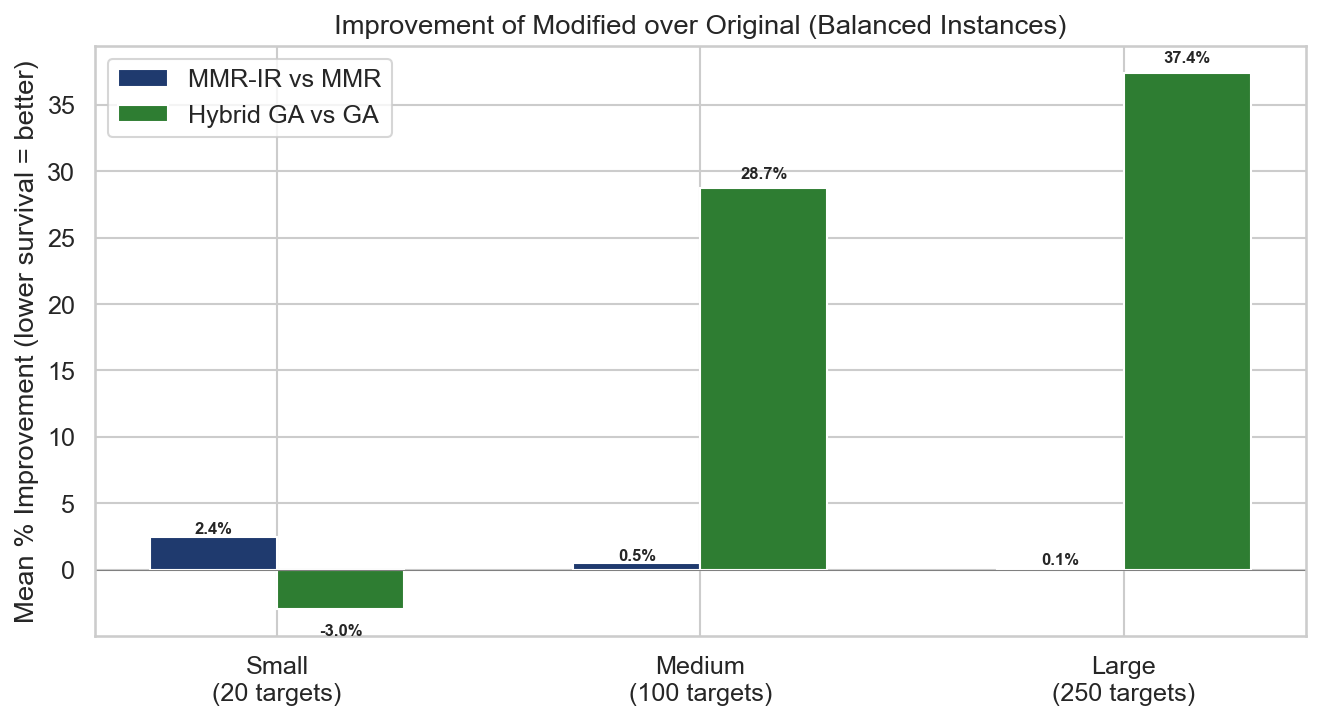
\includegraphics[width=\columnwidth]{03_bar_improvement.png}
  \caption{Percentage improvement of modified algorithms over their baselines,
    broken down by problem size tier (balanced scenario).}
  \label{fig:imp_tier}
\end{figure}


Figure~\ref{fig:imp_tier} confirms that MMR-IR remains positive in every
balanced tier, while Hybrid GA is mixed in small tier and strongly positive in
medium and large tiers.
Scenario-wise, Hybrid GA is positive in all medium/large categories and mixed
in small categories (small\_balanced and small\_scarce are negative, small\_rich
is positive).  MMR-IR remains positive in all nine categories.
\FloatBarrier

\subsection{Runtime Scalability}

Figure~\ref{fig:runtime} shows that on a log-log scale, MMR and MMR-IR remain
orders of magnitude faster than GA variants.  GA variants approach their time
budget cap as size grows; Hybrid GA still achieves superior quality within that
same budget due to the warm start and directed search operators.  The log-log
slopes confirm that both MMR and MMR-IR scale sub-quadratically, while GA
variants are dominated by the fixed time budget.
\FloatBarrier


\begin{figure}[!t]
  \centering
  
\includegraphics[width=\columnwidth]{08_bar_scenario_improvement.png}
  \caption{Percentage improvement of modified algorithms over their baselines,
    broken down by scenario type (balanced / scarce / rich), averaged across
    tiers.}
  \label{fig:imp_scenario}
\end{figure}

% ── Fig 5: Log-log runtime (full width) ──────────────────────────────────────
\begin{figure}[!t]
  \centering
  
\includegraphics[width=\columnwidth]{04_line_time_scalability.png}
  \caption{Mean runtime (seconds) on a log-log scale.  MMR and MMR-IR remain
    orders of magnitude faster than GA variants at all sizes.  GA variants
    approach the time budget as size grows, while Hybrid GA still returns
    superior quality within the same budget.}
  \label{fig:runtime}
\end{figure}

\subsection{Scenario Sensitivity and Scaling Behaviour}

Figure~\ref{fig:scenario} shows that the difficulty ranking across scenarios is
consistent at every tier: scarce (hardest) $>$ balanced $>$ rich (easiest).
This validates the dataset design.  Hybrid GA consistently dominates GA
(original) in medium and large tiers across scenarios; small-tier outcomes are
mixed.

\subsubsection*{Scaling Gain by Problem Size}



Figure~\ref{fig:scale_ga} and Figure~\ref{fig:scale_mmr} isolate the scaling
behaviour of each modification.
Hybrid GA's advantage grows sharply with problem size, confirming that the
three modifications jointly address the scalability bottleneck of standard GA.
MMR-IR shows a stable positive trend at every scale.
\FloatBarrier


% ── Fig 6: Scenario comparison (full width) ───────────────────────────────────
\begin{figure*}[!t]
  \centering
  
\includegraphics[width=\textwidth]{06_scenario_comparison.png}
  \caption{Mean objective value broken down by scenario type (balanced, scarce,
    rich) and tier.  The scarce scenario consistently produces the highest
    residual survival; the rich scenario the lowest.  Algorithm rankings are
    stable across all conditions.}
  \label{fig:scenario}
\end{figure*}

% ── Fig 7a: Scaling gain (Hybrid GA) ──────────────────────────────────────────
\begin{figure*}[!t]
  \centering
  \subfloat[Hybrid GA over GA.\label{fig:scale_ga}]{%
    
\includegraphics[width=0.49\textwidth]{09_ga_improvement_vs_size.png}}%
  \hfill%
% ── Fig 7b: Scaling gain (MMR-IR) ─────────────────────────────────────────────
  \subfloat[MMR-IR over MMR.\label{fig:scale_mmr}]{%
    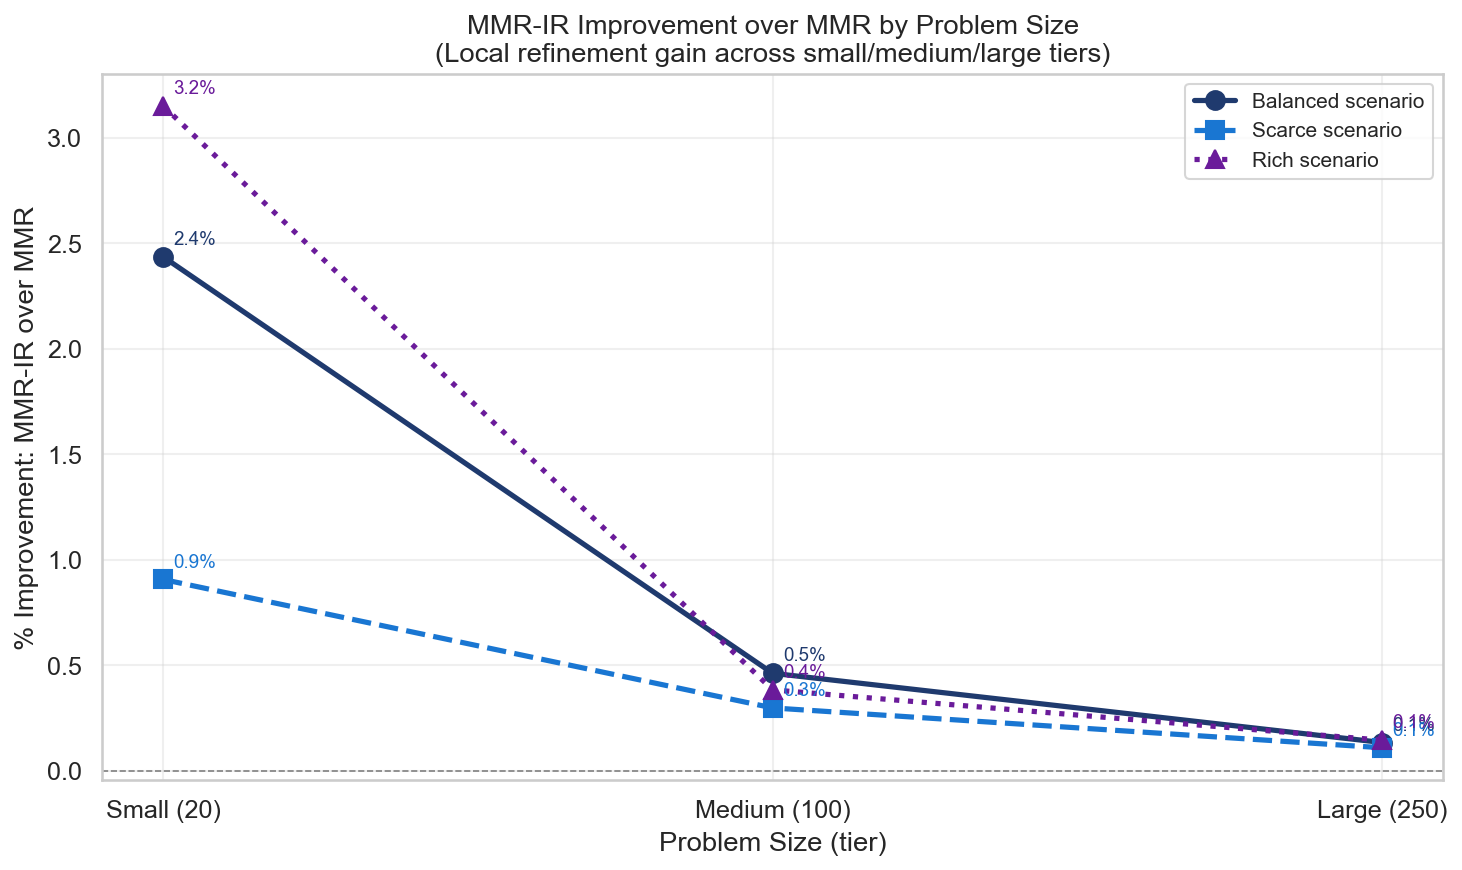
\includegraphics[width=0.49\textwidth]{10_mmr_improvement_vs_size.png}}
  \caption{Scaling comparison by problem size.  Hybrid GA shows a strong
    scale-amplified gain; MMR-IR remains positive and steadier across scales.}
\end{figure*}

\subsection{Why GA (Original) Underperforms at Scale}

At large tier ($W = 375$, $T = 250$), the standard GA population size is
$\max(375, 250) = 375$.  Even with a 60-second budget, the algorithm still
explores only a tiny fraction of the $T^W$ search space from a purely random
start.  Combined with the
absence of elitism (the best solution can be overwritten) and uniform mutation
(ignoring high-threat targets), the standard GA rarely converges near the
MMR-greedy solution, let alone beyond it.

Hybrid GA resolves each of these issues directly:
MMR seeding provides a strong individual from generation 0;
elitism ensures this individual persists;
stagnation-triggered re-diversification helps prevent premature convergence;
and threat-proportional mutation focuses every mutation step on the most
impactful assignments.

The symmetric flip on small-tier instances is equally explicable.
With $\max(W,T)=20$, the GA population has only 20 individuals and a
5-second budget that is sufficient for the standard GA to converge by
random exploration alone.
MMR seeding concentrates initial diversity into one greedy individual,
and 10\% elitism (2 out of 20) creates disproportionate selection pressure.
The result is reduced exploration in an already-small search space, causing
Hybrid GA to perform comparably to or slightly worse than the standard GA
on these easy instances.
This is consistent with the non-significant Wilcoxon results for all three
small-tier categories.

\subsection{Statistical Significance}

Using the one-sided Wilcoxon signed-rank test
(``original $>$ modified'', $\alpha = 0.05$):
\begin{itemize}
  \item \textbf{MMR-IR vs.\ MMR} is significant in all $9/9$ categories.
  \item \textbf{Hybrid GA vs.\ GA} is significant in $6/9$ categories.
  \item The three non-significant categories are all small-tier:
        small\_balanced ($p=0.9932$), small\_scarce ($p=0.9978$),
        and small\_rich ($p=0.1650$).
\end{itemize}

% ─────────────────────────────────────────────────────────────────────────────
\section{Conclusion}
\label{sec:conclusion}

This paper addressed the Weapon-Target Assignment problem from an algorithm
engineering perspective, identifying structural weaknesses in two well-studied
baseline approaches — MMR and standard GA — and proposing targeted
modifications that empirically improve performance on a controlled synthetic
benchmark.

\textbf{MMR-IR} augments the greedy heuristic with tie-aware allocation and
two local-search phases (1-opt and 2-opt) using $O(1)$ incremental
evaluation.  On balanced tiers, it improves MMR by 2.44\%, 0.46\%, and
0.13\% (small/medium/large), and remains statistically significant in all
9 categories.

\textbf{Hybrid GA} directly addresses the three failure modes of standard GA
on large WTA instances --- random initialisation, solution loss, and uninformed
mutation --- through MMR seeding, elitism with stagnation-triggered
re-diversification, and the
threat-proportional mutation operator.  On balanced tiers, it changes
GA performance by -2.95\%, 28.73\%, and 37.42\% (small/medium/large).  The
method is strongly effective in medium/large categories and significant in
6 of 9 categories overall.

Together, the two modifications improve the quality-runtime trade-off from
different directions: MMR-IR provides consistent incremental gain at near-greedy
speed, while Hybrid GA provides major gains where instance scale is large
enough for guided evolutionary search to pay off.

\textbf{Limitation.} The evaluation uses a synthetic 180-instance benchmark and
compares against standard MMR and GA baselines.  The results therefore support
claims about controlled comparative performance on this benchmark, not blanket
claims of superiority over all exact, heuristic, or metaheuristic approaches.

\textbf{Future directions.} Promising extensions include coupling MMR-IR as a
local-search operator within Hybrid GA (a memetic GA), exploring adaptive
time-budget allocation that scales with instance hardness, and evaluating the
modifications on dynamic WTA variants where targets arrive in real time.

% ─────────────────────────────────────────────────────────────────────────────
\section*{Reproducibility}

All code, datasets, and instructions are available at:
\begin{center}
  \url{https://github.com/Arimotokika/CSE_462-Algorithm-Engineering-Sessional}
\end{center}
All 180 instances, the four algorithm implementations, and the analysis
pipeline are reproduced by executing the single master script:
\begin{center}
  \texttt{cd codes}\\
  \texttt{pip install -r requirements.txt}\\
  \texttt{python run\_all.py}
\end{center}
On our setup, full reproduction takes approximately 3--4 hours
(large-tier categories dominate runtime).

\clearpage

% ─────────────────────────────────────────────────────────────────────────────
\IEEEtriggeratref{10}
\IEEEtriggercmd{\enlargethispage{-5in}}
\begin{thebibliography}{15}
\bibitem{kline2020} A.~G. Kline, D.~K. Ahner, and B.~J. Lunday, ``A heuristic and metaheuristic approach to the static weapon target assignment problem,'' \textit{Journal of Global Optimization}, vol.~78, no.~4, pp.~791--812, 2020.
\bibitem{ahuja2007} R.~K. Ahuja, A.~Kumar, K.~Jha, and J.~B. Orlin, ``Exact and heuristic algorithms for the weapon-target assignment problem,'' \textit{Operations Research}, vol.~55, no.~6, pp.~1136--1146, 2007.
\bibitem{lloyd1986} S.~P. Lloyd and H.~S. Witsenhausen, ``Weapons allocation is NP-complete,'' in \textit{Proc. Summer Computer Simulation Conference}, pp.~1054--1058, 1986.
\bibitem{bertsimas2025} D.~Bertsimas and A.~Paskov, ``Solving large-scale weapon target assignment problems in seconds using branch-price-and-cut,'' \textit{Naval Research Logistics}, vol.~72, no.~5, pp.~735--749, 2025.
\bibitem{andersen2022} A.~C. Andersen, K.~Pavlikov, and T.~A.~M. Toffolo, ``Weapon-target assignment problem: exact and approximate solution algorithms,'' \textit{Annals of Operations Research}, vol.~312, no.~2, pp.~581--606, 2022.
\bibitem{kwon1999} O.~Kwon, K.~Lee, and D.~Park, ``A Lagrangian relaxation approach to the targeting problem,'' \textit{Naval Research Logistics}, vol.~46, no.~7, pp.~640--653, 1999.
\bibitem{kim2022} Y.~Kim, J.~Cho, S.~Han, and N.~Cho, ``Weapon target assignment model for small unit ground combat using mixed integer nonlinear program and Lagrangian relaxation,'' \textit{Mathematical Problems in Engineering}, vol.~2022, pp.~1--13, 2022.
\bibitem{sonuc2020} E.~Sonuc and B.~Sen, ``Weapon target assignment problem,'' in \textit{Artificial Intelligence --- Applications in Military Science}, IntechOpen, 2020.
\bibitem{xin2018} B.~Xin, Y.~Wang, and J.~Chen, ``An efficient marginal-return-based constructive heuristic to solve the sensor-weapon-target assignment problem,'' \textit{IEEE Transactions on Systems, Man, and Cybernetics: Systems}, vol.~49, no.~12, pp.~2536--2547, 2019.
\bibitem{bogdanowicz2013} Z.~R. Bogdanowicz, A.~Tolano, K.~Patel, and N.~P. Coleman, ``Optimization of weapon-target pairings based on kill probabilities,'' \textit{IEEE Transactions on Cybernetics}, vol.~43, no.~6, pp.~1835--1844, 2013.
\bibitem{lee2003} Z.~J. Lee and W.~L. Lee, ``A hybrid search algorithm of ant colony optimization and genetic algorithm applied to weapon-target assignment problems,'' in \textit{Proc. 4th Int.\ Conf.\ Intelligent Data Engineering and Automated Learning (IDEAL)}, Springer, pp.~278--285, 2003.
\bibitem{lee2002} Z.~J. Lee, C.~Y. Lee, and S.~F. Su, ``An immunity-based ant colony optimization algorithm for solving weapon-target assignment problem,'' \textit{Applied Soft Computing}, vol.~2, no.~1, pp.~39--47, 2002.
\bibitem{hu2018} X.~Hu, P.~Luo, X.~Zhang, and J.~Wang, ``Improved ant colony optimization for weapon-target assignment,'' \textit{Mathematical Problems in Engineering}, vol.~2018, pp.~1--14, 2018.
\bibitem{li2017} Y.~Li, Y.~Kou, Z.~Li, A.~Xu, and Y.~Chang, ``A modified Pareto ant colony optimization approach to solve biobjective weapon-target assignment problem,'' \textit{International Journal of Aerospace Engineering}, vol.~2017, pp.~1--14, 2017.
\bibitem{lu2024} J.~Lu, X.~Liang, X.~Chen, and Y.~Ding, ``A comprehensive survey of weapon target assignment problem: Model, algorithm, and application,'' \textit{Engineering Applications of Artificial Intelligence}, vol.~137, p.~109212, 2024.
\end{thebibliography}

\end{document}
